\subsection{Kalibrierung der großen Scheibe}
Mit der großen Scheibe funktioniert die für die Winkelrichtgröße $D$ genauso wie für die kleine Scheibe. Aus diesem Grund werden hier nur die Werte (inkl. Fehler) angegeben. Es ergibt sich folgender Wert (Daten, siehe Abb. \ref{fig:kal2})
\begin{align*}
D = \unit[(2.17 \pm 0.04)]{N m}
\end{align*}
Die großen Fehlerwerte ergeben sich dadurch, dass die rücktreibende Kraft von der Richtung, in die die Scheibe ausgelenkt wird abhängt (materialbedingt).

\begin{figure}
\begin{center}
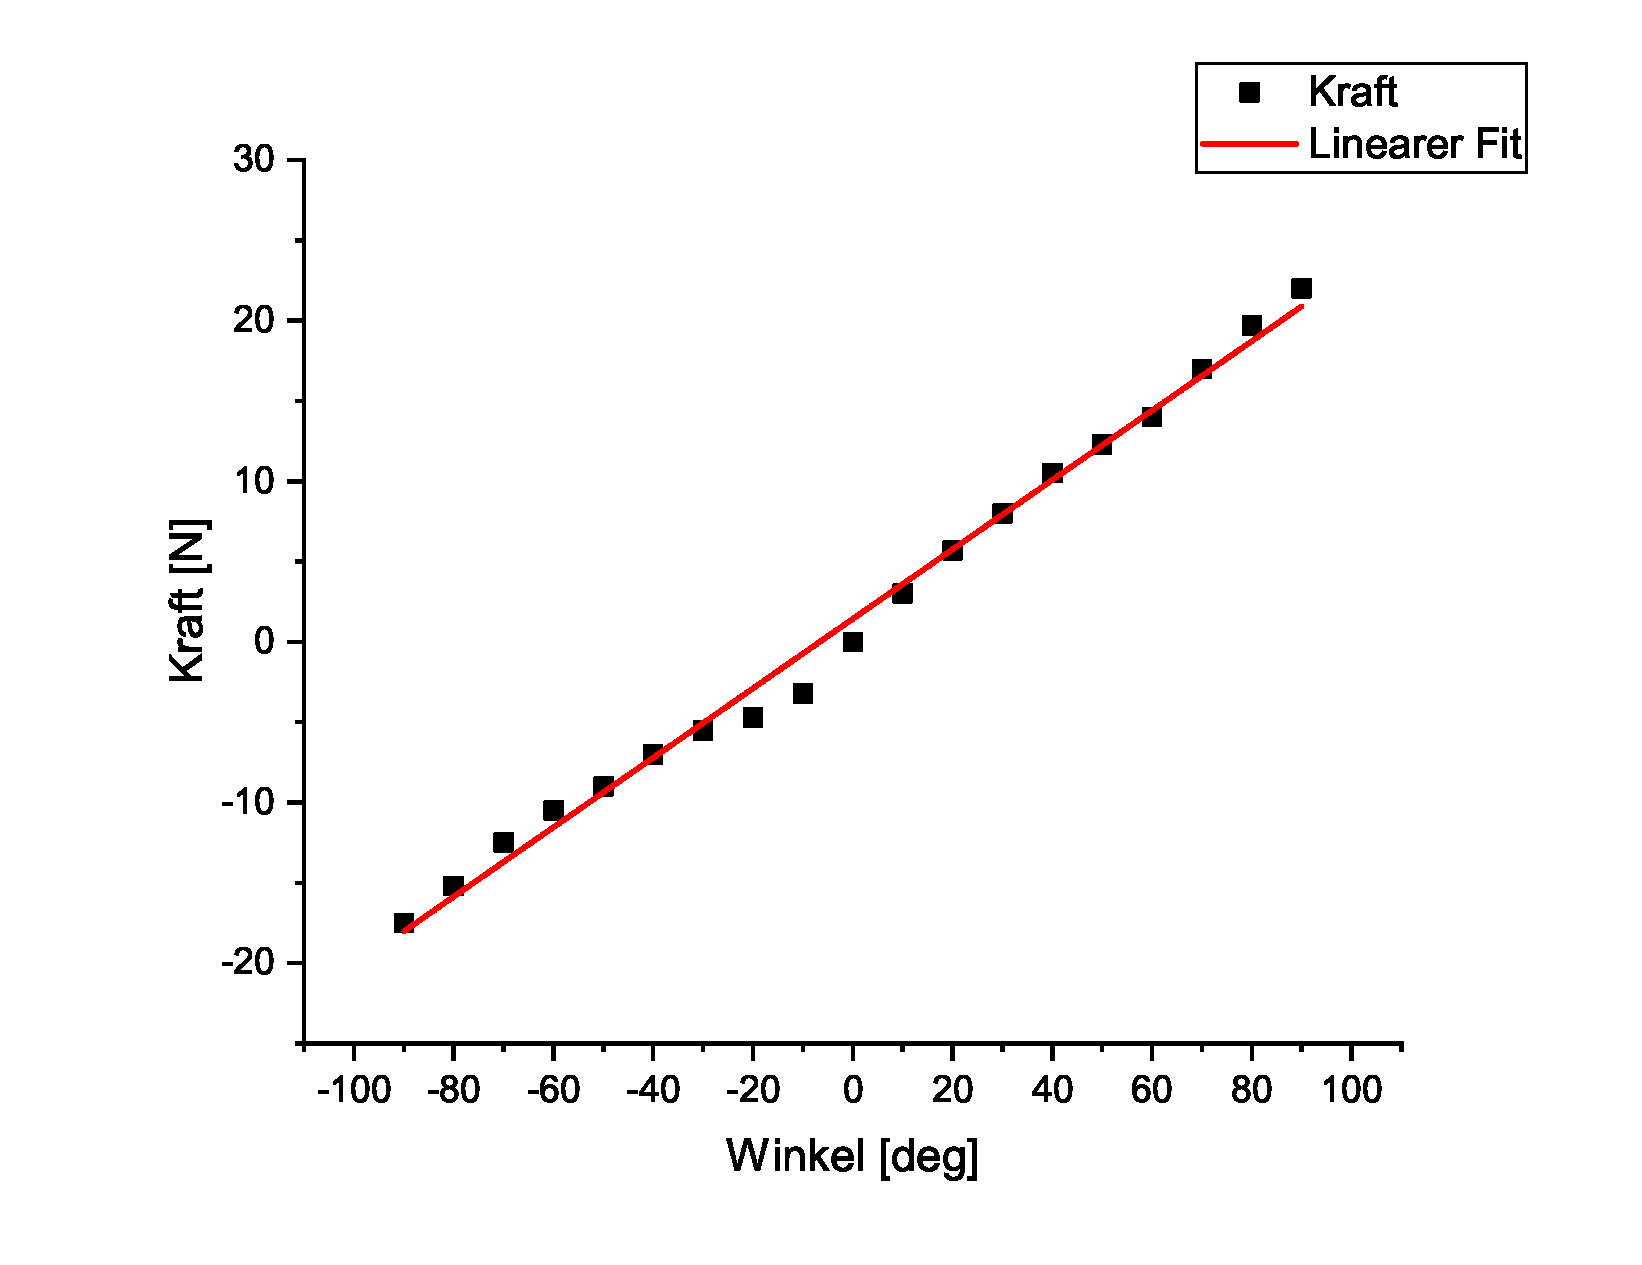
\includegraphics[width=0.7\textwidth]{Bilder/kal2.eps}
\caption{Kalibrierung der großen Scheibe}
\label{fig:kal2}
\end{center}
\end{figure}